% !TeX root = ../index.tex
\chapter{Syntax}
\graphicspath{{2-syntax/images/}}

\section{Exercise 1}

Converted the shorthand PHP tags (\texttt{<?...?>}) to \texttt{<?php...?>} as IntWeb has disabled the language feature.

\url{https://intweb.bucks.ac.uk/~21606555/oos/2-syntax/ex1.php}
\captionsetup{type=figure}\captionof{figure}{ex1.php}
\subfile{pyg/src/2-syntax/ex1}

\begin{figure}[H]
  \caption{Output of exercise 1}
  \centering
  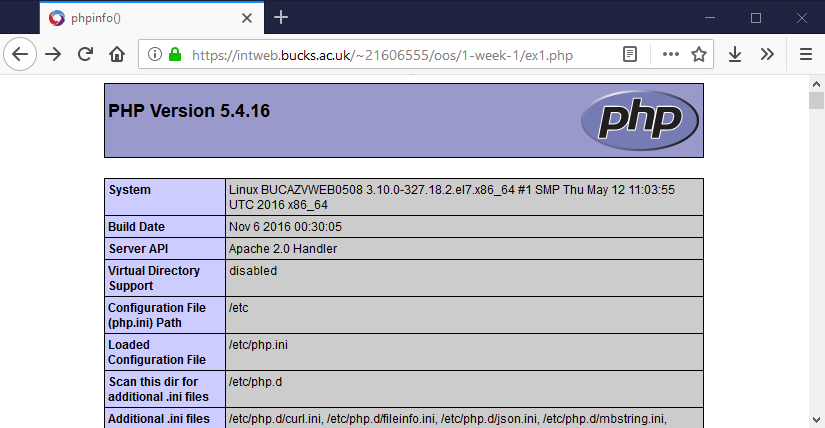
\includegraphics[width=\textwidth]{ex1}
\end{figure}

\clearpage
\section{Exercise 2}

\url{https://intweb.bucks.ac.uk/~21606555/oos/2-syntax/ex2.php}
\captionsetup{type=figure}\captionof{figure}{ex2.php}
\subfile{pyg/src/2-syntax/ex2}

\begin{figure}[H]
  \caption{Output of exercise 2}
  \centering
  \includegraphics[width=\textwidth]{ex2}
\end{figure}

\clearpage
\section{Exercise 3}

\url{https://intweb.bucks.ac.uk/~21606555/oos/2-syntax/ex3.php}
\captionsetup{type=figure}\captionof{figure}{ex3.php}
\subfile{pyg/src/2-syntax/ex3}

\begin{figure}[H]
  \caption{Output of exercise 3}
  \centering
  \includegraphics[width=\textwidth]{ex3}
\end{figure}

\clearpage
\section{Exercise 4}

\url{https://intweb.bucks.ac.uk/~21606555/oos/2-syntax/ex4.php}
\captionsetup{type=figure}\captionof{figure}{ex4.php}
\subfile{pyg/src/2-syntax/ex4}

\begin{figure}[H]
  \caption{Output of exercise 4}
  \centering
  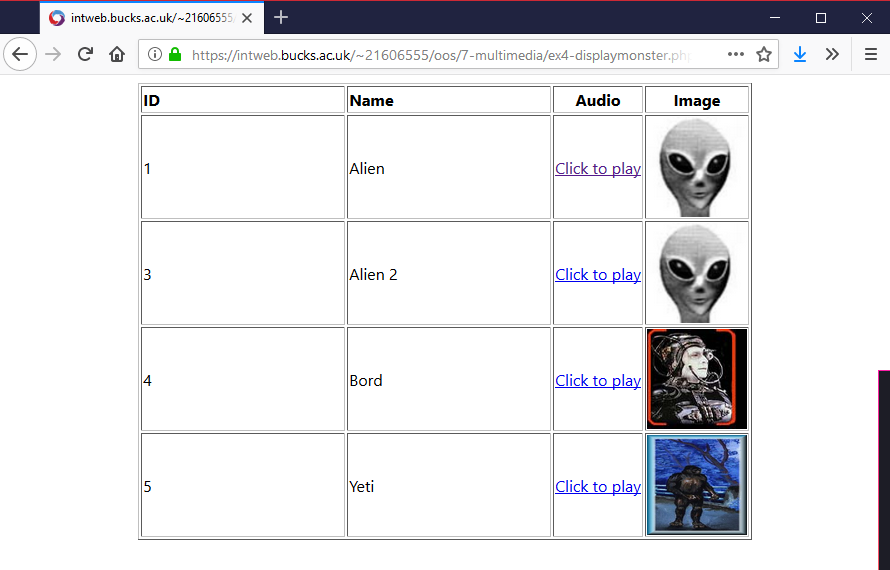
\includegraphics[width=\textwidth]{ex4}
\end{figure}

\clearpage
\section{Exercise 5}

\url{https://intweb.bucks.ac.uk/~21606555/oos/2-syntax/ex5.php}
\captionsetup{type=figure}\captionof{figure}{ex5.php}
\subfile{pyg/src/2-syntax/ex5}

\begin{figure}[H]
  \caption{Output of exercise 5}
  \centering
  
\includegraphics[width=\textwidth]{ex5}
\end{figure}

\clearpage
\section{Exercise 6}

If an index position isn't specified when assigning a value to an array then the value is inserted after the last index position in the array. In this case, $76$ is inserted into the 4th index.\\

\url{https://intweb.bucks.ac.uk/~21606555/oos/2-syntax/ex6.php}
\captionsetup{type=figure}\captionof{figure}{ex6.php}
\subfile{pyg/src/2-syntax/ex6}

\begin{figure}[H]
  \caption{Output of exercise 6}
  \centering
  
\includegraphics[width=\textwidth]{ex6}
\end{figure}

\clearpage
\section{Exercise 7}

11 lines will be displayed as it will loop from 0 until it reaches 10.\\

\url{https://intweb.bucks.ac.uk/~21606555/oos/2-syntax/ex7.php}
\captionsetup{type=figure}\captionof{figure}{ex7.php}
\subfile{pyg/src/2-syntax/ex7}

\begin{figure}[H]
  \caption{Output of exercise 7}
  \centering
  \includegraphics[width=\textwidth]{ex7}
\end{figure}

\clearpage
\section{Exercise 8}

Fixed the for loop syntax where a comma was used instead of a semi-colon.\\

\url{https://intweb.bucks.ac.uk/~21606555/oos/2-syntax/ex8.php}
\captionsetup{type=figure}\captionof{figure}{ex8.php}
\subfile{pyg/src/2-syntax/ex8}

\begin{figure}[H]
  \caption{Output of exercise 8}
  \centering
  \includegraphics[width=\textwidth]{ex8}
\end{figure}

\clearpage
\section{Exercise 9}

\url{https://intweb.bucks.ac.uk/~21606555/oos/2-syntax/ex9.php}
\captionsetup{type=figure}\captionof{figure}{ex9.php}
\subfile{pyg/src/2-syntax/ex9}

\begin{figure}[H]
  \caption{Output of exercise 9}
  \centering
  \includegraphics[width=\textwidth]{ex9}
\end{figure}

\clearpage
\section{Exercise 10}

This has been revised to be displayed in a table from the exercise 12 task.\\

\url{https://intweb.bucks.ac.uk/~21606555/oos/2-syntax/ex10.php}
\captionsetup{type=figure}\captionof{figure}{ex10.php}
\subfile{pyg/src/2-syntax/ex10}

\begin{figure}[H]
  \caption{Output of exercise 10}
  \centering
  \includegraphics[width=\textwidth]{ex10}
\end{figure}

\clearpage
\section{Exercise 11}

I opted to use the \texttt{sizeof} function to calculate the averages so that the average will always be correct if marks are removed or added to the array.\\

\url{https://intweb.bucks.ac.uk/~21606555/oos/2-syntax/ex11.php}
\captionsetup{type=figure}\captionof{figure}{ex11.php}
\subfile{pyg/src/2-syntax/ex11}

\begin{figure}[H]
  \caption{Output of exercise 11}
  \centering
  \includegraphics[width=\textwidth]{ex11}
\end{figure}

\clearpage
\section{Exercise 12}

\url{https://intweb.bucks.ac.uk/~21606555/oos/2-syntax/ex12.php}
\captionsetup{type=figure}\captionof{figure}{ex12.php}
\subfile{pyg/src/2-syntax/ex12}

\begin{figure}[H]
  \caption{Output of exercise 12}
  \centering
  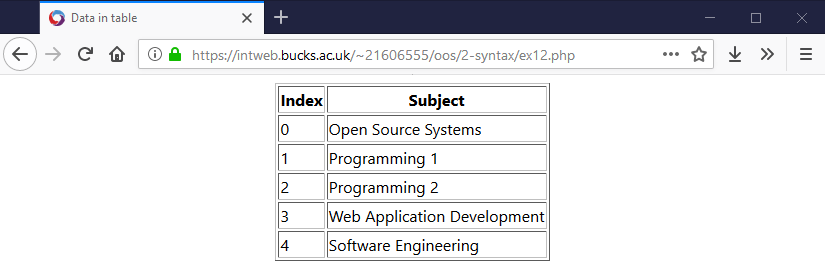
\includegraphics[width=\textwidth]{ex12}
\end{figure}
